\documentclass[submission]{eptcs}
\providecommand{\event}{TTC 2015}

\usepackage[T1]{fontenc}
\usepackage{varioref}
\usepackage{hyperref}

\usepackage{url}
\usepackage{paralist}
\usepackage{graphicx}
\usepackage[cache]{minted}
\newminted{clojure}{fontsize=\fontsize{8}{8},linenos,numbersep=3pt,numberblanklines=false}
\newmintinline{clojure}{fontsize=\small}
\newcommand{\code}{\clojureinline}
\VerbatimFootnotes

\title{Solving the TTC Java Refactoring Case with FunnyQT}
\author{Tassilo Horn
  \institute{Institute for Software Technology, University Koblenz-Landau, Germany}
  \email{horn@uni-koblenz.de}}

\def\titlerunning{Solving the TTC Java Refactoring Case with FunnyQT}
\def\authorrunning{T. Horn}

\begin{document}
\maketitle

\begin{abstract}
  This paper describes the FunnyQT solution to the TTC 2015 Java Refactoring
  transformation case.  The solution solves all core tasks and also the
  extension tasks 1 and 2, and it has been selected as overall winner of this
  case.
\end{abstract}


\section{Introduction}
\label{sec:introduction}

This paper describes the FunnyQT\footnote{\url{http://funnyqt.org}}
~\cite{Horn2013MQWFQ,funnyqt-icgt15} solution of the TTC 2015 Java Refactoring
Case~\cite{java-refactoring-case-desc}.  It solves all core and exception tasks
with the exception of \emph{Extension~3: Detecting Refactoring Conflicts}.  The
solution project is available on
Github\footnote{\url{https://github.com/tsdh/ttc15-java-refactoring-funnyqt}},
and it is set up for easy reproduction on a SHARE image\footnote{The SHARE
  image name is \verb|ArchLinux64_TTC15-FunnyQT_2|}.

FunnyQT is a model querying and transformation library for the functional Lisp
dialect Clojure\footnote{\url{http://clojure.org}}.  Queries and
transformations are Clojure programs using the features provided by the FunnyQT
API.

Clojure provides strong metaprogramming capabilities that are used by FunnyQT
in order to define several \emph{embedded domain-specific languages} (DSL) for
different querying and transformation tasks.

FunnyQT is designed with extensibility in mind.  By default, it supports EMF
models and JGraLab TGraph models.  Support for other modeling frameworks can be
added without having to touch FunnyQT's internals.

The FunnyQT API is structured into several namespaces, each namespace providing
constructs supporting concrete querying and transformation use-cases, e.g.,
model management, pattern matching, out-place transformations, in-place
transformations, bidirectional transformations, and some more.  For solving
this case, FunnyQT's out-place and in-place transformation DSLs have been used.


\section{Solution Description}
\label{sec:solution-description}

\subsection{Step 1: Java Code to Program Graph}
\label{sec:step-1:java-to-pg}

The first step in the transformation chain is to create an instance model
conforming to the program graph metamodel predefined in the case description
from the Java source code that should be subject to refactoring.  The FunnyQT
solution does that in two substeps.

\begin{compactenum}[(a)]
\item Parse the Java source code into a model conforming to the EMFText
  JaMoPP\footnote{\url{http://www.jamopp.org/index.php/JaMoPP}} metamodel.
\item Transform the JaMoPP model to a program graph metamodel using a FunnyQT
  out-place transformation.
\end{compactenum}

Step (a) is implemented in the solution namespace
\emph{ttc15-java-refactoring-funnyqt.jamopp}.  It simply sets up JaMoPP and
defines two functions \code|parse-directory| and \code|save-java-rs|.  The
former parses all Java files contained in the given directory and returns a
resource set representing the sources' abstract syntax graph conforming to the
JaMoPP metamodel.  The second function receives such a resource set and saves
it back as Java code.  Both just access JaMoPP built-in functionality.

Step (b) is implemented as a FunnyQT out-place transformation in the solution
namespace \emph{ttc15-java-refactoring-funnyqt.jamopp2pg}.  It creates a
program graph model from the JaMoPP model.

The transformation also minimizes the target program graph.  The source JaMoPP
model contains the complete syntax graph of the parsed Java sources including
all dependencies of those.  I.e., if the parsed Java program uses the
\textsf{java.util.List} interface, then the JaMoPP model also contains this
interface's ASG, i.e., all its declared methods, its super-interfaces, etc.
The program graph created by the transformation only contains \textsf{TClass}
elements for the Java classes parsed from source code and direct dependencies
used as field type or method parameter or method return type.  \textsf{TMember}
elements are only created for the methods of directly parsed Java classes, and
then only for those members that are not static because the case description
explicitly excluded statics.  As a result, the program graph contains only the
information relevant to the refactorings and is reasonably small so that it can
be visualized which is nice especially for debugging.

The FunnyQT out-place transformation API used for implementing this task is
quite similar to ATL or QVT Operational Mappings.  There are mapping rules
which receive one or many JaMoPP source elements and create one or many target
program graph elements.

A cutout of the transformation depicting the rules responsible for transforming
fields is given in the following listing.  The transformation receives one
single source model \code|jamopp| and one single target model \code|pg|.

\begin{clojurecode}
(deftransformation jamopp2pg [[jamopp] [pg]]
  ...
  (field2tfielddef
   :from [f 'Field]
   :when (not (static? f))
   :to   [tfd 'TFieldDefinition {:signature (get-tfieldsig f)}])
  (get-tfieldsig
   :from [f 'Field]
   :id   [sig (str (type-name (get-type f)) " " (j/name f))]
   :to   [tfs 'TFieldSignature {:field (get-tfield f)
                                :type  (type2tclass (get-type f))}])
  (get-tfield
   :from [f 'Field]
   :id   [n (j/name f)]
   :to   [tf 'TField {:tName n}]
   (pg/->add-fields! *tg* tf))
  (type2tclass
   :from [t 'Type]
   :disjuncts [class2tclass primitive2tclass])
  ...)
\end{clojurecode}

For each non-static field (declared by a user-defined class) in the JaMoPP
model, the \code|field2tfielddef| rule creates a \textsf{TFieldDefinition}
element in the program graph.  The signature of this \textsf{TFieldDefinition}
is set to the result of calling the \code|get-tfieldsig| rule.

This rule uses the \code|:id| feature to implement a n:1 semantics.  Only for
each unique string \code|sig| created by concatenating the field's type and
name, a new \textsf{TFieldSignature} is created.  If the rule is called
thereafter for some other field with the same type and name, the existing field
signature created at the first call is returned.  The field signature's
\textsf{field} and \textsf{type} references pointing to a \textsf{TField} and a
\textsf{TClass} respectively are set by calling the \code|get-tfield| and
\code|type2tclass| rules.

The \code|get-tfield| is again a n:1 rule creating a \textsf{TField} element
for every unique field name.  The \code|type2tclass| rule is a disjunctive rule
that delegates to either \code|class2tclass| or \code|primitive2tclass| to
create a (or retrieve an existing) \textsf{TClass} for a given JaMoPP class or
primitive type.

Note that in the rules above, the name of a field is retrieved using
\code|(j/name f)|.  This is because the solution lets FunnyQT generate
metamodel-specific APIs for both the JaMoPP and program graph metamodels into
two namespaces which are required with the aliases \code|j| and \code|pg|
respectively.  These generated APIs contain attribute accessor functions
(e.g. \code|(j/name x)| and \code|(j/set-name! x val)|), reference accessors
(e.g., \code|(pg/->access tdef)|, \code|(pg/->set-access! tdef accs)|,
\code|(pg/->add-access! tdef acc)|, and \code|(pg/->remove-access! tdef acc)|),
element constructors (e.g., \code|(pg/create-TClass! model)|), and element
sequence functions (e.g., \code|(pg/all-TClasses model)|).  The functions of
the generated APIs allow for a bit more conciseness and a better readability
than the generic accessor functions.  With the latter, the name of a JaMoPP
field would be retrieved using \code|(eget f :name)|.

In total, the transformation consists of 10 rules summing up to 71 lines of
code.  In addition, there are five simple helper functions like \code|static?|,
\code|get-type|, and \code|type-name| that have been used in the above rules
already.

\bigskip{}

A FunnyQT transformation like the one briefly discussed above returns a map of
traceability information.  This map's keys are the transformation rules, and
the values are maps from the respective rule's input elements to its output
elements.  For the third step of the overall transformation, i.e., the
back-propagation of the changes performed in the program graph to the Java
source code, we only need to be able to get from a program graph
\textsf{TClass} to the corresponding JaMoPP \textsf{Class}, from a program
graph \textsf{TFieldDefinition} to the corresponding JaMoPP \textsf{Field}, and
from a program graph \textsf{TMethodDefinition} to the corresponding JaMoPP
\textsf{ClassMethod}.  I.e., we need an inverse lookup from target to source
elements, and we are not interested in which rule created what element.  Thus,
the following helper function \code|prepare-pg2jamopp-ma| creates such an
inverse lookup map from the given transformation trace.

\begin{clojurecode}
(defn prepare-pg2jamopp-map [trace]
  (atom (into {} (comp (map #(% trace))
                       (map set/map-invert))
              [:class2tclass :field2tfielddef :method2tmethoddef])))
\end{clojurecode}

The function also wraps the inverse lookup map in a Clojure \emph{atom}.  All
Clojure data structures such as lists, vectors, or maps are immutable.
However, during (multi-step) refactoring we need to be able to update the
inverse lookup map.  Atoms are atomically mutable references to immutable data
structures.  Thus, during refactoring, the reference to the inverse lookup map
can be changed atomically to a new map reflecting an updated inverse lookup
map.


\subsection{Step~2: Refactoring of the Program Graph}
\label{sec:step-2:refactoring-pg}

The refactorings are implemented in the solution namespace
\emph{ttc15-java-refactoring-funnyqt.refactor} using FunnyQT in-place
transformation rules which combine patterns to be matched in the model with
actions to be applied to the matched elements.

Before discussing the rules, the following two helper functions need to be
discussed.

\begin{clojurecode}
(defn find-tclass [pg qn]
  (first (filter #(= qn (pg/tName %))
                 (pg/all-TClasses pg))))

(defn find-tmethodsig [pg method-name param-qns]
  (let [pclasses (mapv (partial find-tclass pg) param-qns)]
    (first (filter #(and (-> % pg/->method pg/tName (= method-name))
                         (= pclasses (pg/->paramList %)))
                   (pg/all-TMethodSignatures pg)))))
\end{clojurecode}

The function \code|find-tclass| receives the program graph \code|pg| and a
qualified name \code|qn| and returns the \textsf{TClass} with this qualified
name.  \code|find-tmethodsig| receives the program graph \code|pg|, a
\code|method-name|, and a sequence of the method's parameter qualified names
\code|param-qns|.  It returns the \code|TMethodSignature| specified by this
combination of method name and parameter types.

These two functions are called by the solution's \textsf{TestInterface}
implementation class in order to have the actual refactoring rules parametrized
with program graph elements instead of the ARTE classes
\code|Pull_Up_Refactoring| and the like.


\paragraph{Pull Up Member.}

The case description requests \emph{pull-up method} as first refactoring core
task.  However, with respect to the program graph metamodel, there is actually
no difference in pulling up a method (\textsf{TMethodDefinition}) or a field
(\textsf{TFieldDefinition}), i.e., it is possible to define the refactoring
more general as \emph{pull-up member} (\textsf{TMember}) and have it work for
both fields and methods.  This is what the FunnyQT solution does.

The corresponding \code|pull-up-member| rule is shown in the next listing.  The
rule is overloaded on arity.  There is the version (1) of arity three which
receives the program graph \code|pg|, the inverse lookup map atom
\code|pg2jamopp-map-atom|, and the JaMoPP resource set \code|jamopp|, and there
is the version (2) of arity four which receives the program graph \code|pg|,
the inverse lookup map atom \code|pg2jamopp-map-atom|, a \textsf{TClass}
\code|super|, and a \textsf{TSignature} \code|sig|.

\begin{clojurecode*}{firstnumber=last}
(defrule pull-up-member
  ([pg pg2jamopp-map-atom jamopp]                                             ;; (1)
   [:extends [(pull-up-member 1)]]                                            ;; pattern
   ((do-pull-up-member! pg pg2jamopp-map-atom super sub member sig others)    ;; action
    jamopp))
  ([pg pg2jamopp-map-atom super sig]                                          ;; (2)
   [super<TClass> -<:childClasses>-> sub -<:signature>-> sig                  ;; pattern
    sub -<:defines>-> member<TMember> -<:signature>-> sig
    :nested [others [super -<:childClasses>-> osub
                     :when (not= sub osub)
                     osub -<:signature>-> sig
                     osub -<:defines>-> omember<TMember> -<:signature>-> sig]]
    :when (seq others)                                                        ;; (a)
    super -!<:signature>-> sig                                                ;; (b)
    :when (= (count (pg/->childClasses super)) (inc (count others)))          ;; (c)
    :when (forall? (partial accessible-from? super)                           ;; (d)
                   (mapcat pg/->access (conj (map :omember others) member)))]
   (do-pull-up-member! pg pg2jamopp-map-atom super sub member sig others)))   ;; action
\end{clojurecode*}

The version (2) is the one which is called by the \textsf{TestInterface}
implementation when being called from ARTE.  We'll discuss this one first.

The pattern of the version (2) matches a subclass \code|sup| of class
\code|super| where \code|sub| defines a \code|member| of the given signature
\code|sig|.  A nested pattern is used to match all other subclasses of
\code|super| which also define a member with that signature.  The constraint
(a) ensures that there are in fact other subclasses declaring a member with
signature \code|sig|.  Then the negative application condition (b) defines that
the superclass \code|super| must not define a member of the given \code|sig|
already.  The constraint (c) ensures that all subclasses define a member of the
given \code|sig|, i.e., not only a subset of all subclasses do so.  Lastly, the
constraint (d) makes sure that all field and method definitions accessed by the
member to be pulled up is already accessible from the superclass.

The helper function \code|accessible-from?| is defined as follows.

\begin{clojurecode*}{firstnumber=last}
(defn accessible-from? [cls m-or-f]
  (let [defining-cls (econtainer m-or-f)]
    (or (= defining-cls cls)                    ;; (i)
        (superclass? defining-cls cls)          ;; (ii)
        (not (superclass? cls defining-cls))    ;; (iii)
        (and (pg/isa-TMethodDefinition? m-or-f) ;; (iv)
             (member? (pg/->signature m-or-f)
                      (pg/->signature cls))
             (superclass? cls defining-cls)))))

(defn superclass? [super sub]
  (loop [sub-super (pg/->parentClass sub)]
    (when sub-super
      (or (= sub-super super)
          (recur (pg/->parentClass sub-super))))))
\end{clojurecode*}

It receives a \textsf{TClass} \code|cls| and a \textsf{TMember}
\textsf{m-or-f}.  It returns true only if the given member is accessible from
the given class.  To decide that, it first computes the \textsf{TClass}
defining the member.  Then, there are four cases in which \code|m-or-f| is
accessible from \code|cls|:
\begin{inparaenum}[(i)]
\item the member is defined in \code|cls|,
\item \code|cls| inherits the member from a superclass,
\item the defining class and \code|cls| are in no inheritance relationship at
  all, or
\item the member is a method defined in a subclass of \code|cls|, and this
  method overrides a method defined by \code|cls|.
\end{inparaenum}

The pattern of the arity three variant (1) of the \code|pull-up-member| rule
contains just an \code|:extends| clause specifying that its pattern equals the
pattern defined for the arity four variant.  The variant (1) is used by the
extension task~2 where possible refactorings are to be proposed to the user.
The difference between the overloaded versions of the \code|pull-up-member|
rule is that version (1) matches \code|super| and \code|sig| itself whereas
these two elements are parameters provided by the caller in version (2).

When a match is found, both versions of the rule call the function
\code|do-pull-up-member!| which is defined as follows.

\begin{clojurecode*}{firstnumber=last}
(defn do-pull-up-member! [pg pg2jamopp-map-atom super sub member sig others]
  (doseq [o others]                                                 ;; PG modification
    (doseq [acc (find-accessors pg (:omember o))]
      (pg/->remove-access! acc (:omember o))
      (pg/->add-access! acc member))
    (edelete! (:omember o))
    (pg/->remove-signature! (:osub o) sig))
  (pg/->remove-signature! sub sig)
  (pg/->add-defines! super member)
  (pg/->add-signature! super sig)
  (fn [_]                                                           ;; JaMoPP modification
    (doseq [o others]
      (edelete! (@pg2jamopp-map-atom (:omember o)))
      (swap! pg2jamopp-map-atom dissoc (:omember o)))
    (j/->add-members! (@pg2jamopp-map-atom super) (@pg2jamopp-map-atom member))))

(defn find-accessors [pg tmember]
  (filter #(member? tmember (pg/->access %))
          (pg/all-TMembers pg)))
\end{clojurecode*}

It first applies the changes to the program graph by deleting all duplicate
member definitions from all other subclasses of \code|super| and pulling up the
selected member into \code|super|.  It also updates all accessors of the old
members in order to have them access the single pulled up member.  Lastly, it
returns a closure which performs the equivalent changes in the JaMoPP model and
updates the reference to the inverse lookup map when being called.

We return a function encapsulating the changes here instead of simply applying
the changes because the ARTE \textsf{TestInterface} defines that the
back-propagation of changes happens at a different point in time than the rule
application.  Thus, the solution's \textsf{TestInterface} implementation simply
collects the closures returned by appling a rule in a Java collection and
invokes them in its \code|synchronizeChanges()| implementation.

Note that the rule's variant (1) immediately invokes the function returned by
\code|do-pull-up-member!|.  This is because this variant is not called by ARTE
but is intended for extension task~2, and with that there is no need to defer
back-propagation.



\paragraph{Create Superclass.}

The \code|create-superclass| rule uses the same mechanics as the
\code|pull-up-member| rule.  Again, it is overloaded on arity where the first
version is intended for proposing refactorings to a user and the second version
is for being called by ARTE.

\begin{clojurecode*}{firstnumber=last}
(defrule create-superclass
  ([pg pg2jamopp-map-atom jamopp]
   [sig<TSignature>
    :let [classes (filter #(member? sig (pg/->signature %))
                          (remove pg/->parentClass (pg/all-TClasses pg)))
          new-superclass-qn (str (gensym "ext.NewParent"))]
    :when (> (count classes) 1)
    :extends [(create-superclass 1)]]
   ((do-create-superclass! pg pg2jamopp-map-atom classes scs new-superclass-qn)
    jamopp))
  ([pg pg2jamopp-map-atom classes new-superclass-qn]
   [:let [scs (into #{} (map pg/->parentClass) classes)]
    :when (and (= 1 (count scs))
               (not (find-tclass pg new-superclass-qn)))]
   (do-create-superclass! pg pg2jamopp-map-atom classes scs new-superclass-qn)))
\end{clojurecode*}

The second version is called by ARTE with a set of \code|classes| for which a
new superclass with qualified name \code|new-superclass-qn| should be created.
That version's pattern first computes the set of superclasses \code|scs| of the
given classes.  The constraint then ensures that this set contains exactly one
element, and that no class with qualified name \code|new-superclass-qn| already
exists.  The set of superclasses \code|scs| has exactly one element when either
all the given \code|classes| have no superclass\footnote{Then the set
  \code|scs| contains just \code|nil|.} or all the given \code|classes| have
the same superclass.

The first version of the rule matches a \textsf{TSignature} \code|sig| and all
classes with no superclass which define this signature.  The constraint defines
that there must be at least two such classes.  This ensures that a create
superclass refactoring is only suggested to the user if there are at least two
classes with duplicate features which could probably be pulled up in further
refactoring steps.  Lastly, the pattern extends the pattern of the second
version of \code|create-superclass| and thus inherits the additional
\code|:let| binding and \code|:when| constraint defined in there.

The rule's action in both versions is to call \code|do-create-superclass!|
which is defined as given below.

\begin{clojurecode*}{firstnumber=last}
(defn do-create-superclass! [pg pg2jamopp-map-atom classes scs new-superclass-qn]
  (let [new-tclass (pg/create-TClass! pg {:tName new-superclass-qn
                                          :childClasses classes
                                          :parentClass (first scs)})]
    (fn [^ResourceSet rs]
      (let [[pkgs class-name] (let [parts (str/split new-superclass-qn #"\.")]
                                [(butlast parts) (last parts)])
            ^Resource other-r (.get (.getResources rs) 0)
            r (new-resource rs (str (->> other-r .getURI .toFileString
                                         (re-matches #"(.*[/-]src/).*")
                                         second)
                                    (str/join "/" pkgs) "/" class-name ".java"))
            nc (j/create-Class! nil {:name class-name
                                     :annotationsAndModifiers [(j/create-Public! nil)]})
            cu (j/create-CompilationUnit! r {:name (str new-superclass-qn ".java")
                                             :namespaces  pkgs
                                             :classifiers [nc]})]
        (doseq [c classes]
          (j/->set-extends! (@pg2jamopp-map-atom c) (make-type-reference nc)))
        (when-let [parent (first scs)]
          (j/->set-extends! nc (make-type-reference (@pg2jamopp-map-atom parent))))
        (swap! pg2jamopp-map-atom assoc new-tclass nc)))))

(defn make-type-reference [target-class]
  (j/create-NamespaceClassifierReference!
   nil {:namespaces (j/namespaces (econtainer target-class))
        :classifierReferences [(j/create-ClassifierReference!
                                nil {:target target-class})]}))
\end{clojurecode*}

It creates a new \textsf{TClass} of the given \code|new-superclass-qn| in the
program graph, and makes all \code|classes| a subclass of it.  If those had a
common superclass before the refactoring, then this common superclass becomes
the superclass of the newly created class.

The function again returns a closure which performs the same change to the
JaMoPP model when being invoked to the JaMoPP resource set.  Here, the changes
are a bit longish because actually a new resource containing a compilation unit
defining the new class need to be created, and a bit string-matching needs to
be performed to figure out with which file the newly created class has to be
associated in order to make JaMaPP's serialization back to Java work.


\paragraph{Extract Superclass (Extension~1).}

With the \code|pull-up-member| and \code|create-superclass| rules in place,
defining a \code|extract-superclass| rule is simply a matter of composing the
former two as given below.

\begin{clojurecode*}{firstnumber=last}
(defrule extract-superclass [pg pg2jamopp-map-atom jamopp]
  [:extends [(create-superclass 0)]]
  ((create-superclass pg pg2jamopp-map-atom classes new-superclass-qn) jamopp)
  (let [super (find-tclass pg new-superclass-qn)]
    (doseq [sig (filter (fn [sig]
                          (forall? #(member? sig (pg/->signature %)) classes))
                        (pg/all-TSignatures pg))]
      ((pull-up-member pg pg2jamopp-map-atom super sig) jamopp))))
\end{clojurecode*}

The \code|extract-superclass| rule is not overloaded on arity because it is
never called by ARTE.  Instead, it is only called by extension task~2 in order
to propose a refactoring.

Its pattern extends the pattern of the first variant of
\code|create-superclass|.  Remember that this pattern has been defined in such
a way that it matches only a set of at least two classes which have common
features, i.e., classes for which \code|pull-up-member| will probably be
applicable after creating a superclass.  Note that this is slightly incorrect:
\code|extract-superclass| matches a set of classes with common features where
none of them turns out as actually pullable, too.  However, since the
\code|accessible-from?| predicate requires an existing \textsf{TClass} element
in its current form, the specification of the constraint \emph{there are common
  features and at least one of them would be pullable into a new superclass if
  that were created} would require more code.  Thus we have sacrificed a bit
correctness in some corner-cases for conciseness of the solution.

The rule's actions then simply call \code|create-superclass|, and then call
\code|pull-up-member| for each member whose signature is defined by all
subclasses of the newly created superclass.


\paragraph{Propose Refactoring (Extension~2).}

\begin{sloppypar}
  The rules \code|pull-up-member|, \code|create-superclass|, and
  \code|extract-superclass| discussed above already have overloaded versions
  (or just a single version) which match all elements relevant for the
  corresponding refactoring themselves.
\end{sloppypar}

FunnyQT provides a rule combinator \code|interactive-rule| which receives one
or many rules and returns a new rule which shows to the user all applicable
rules and their matches.  The user can then select the rule and the match to be
applied interactively.

The definition for interactive refactoring is given below.

\begin{clojurecode*}{firstnumber=last}
(defn refactor-interactively [pg pg2jamopp-map-atom jamopp]
  ((interactive-rule create-superclass pull-up-member extract-superclass)
   pg pg2jamopp-map-atom jamopp))
\end{clojurecode*}

An interactive rule for \code|create-superclass|, \code|pull-up-member|, and
\code|extract-superclass| is created and immediately applied to the arguments
which the three rules have in common.

\begin{figure}[h!tb]
  \centering
  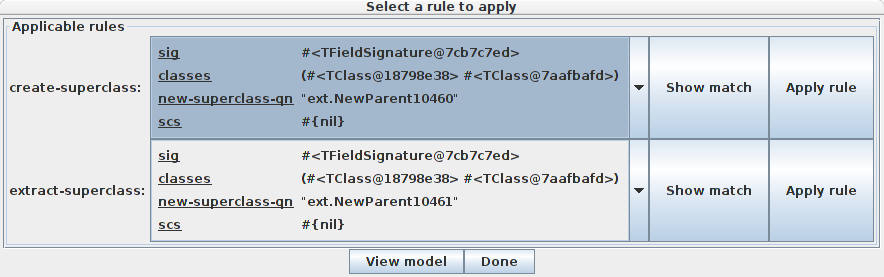
\includegraphics[width=\textwidth]{propose-refactoring}
  \caption{Interactive rule application}
  \label{fig:interactive-rule-application}
\end{figure}

Figure \vref{fig:interactive-rule-application} shows a screenshot of the
interactive rule application GUI.  All applicable rules are listed, and the
match to which a rule should be applied can be selected from comboboxes.  Using
the \emph{View model} and \emph{Show match} buttons, visualizations of the
complete model or only the parts around the currently selected match can be
shown.

This interactive rule application is automatically started when running
\code|lein test| in the solution project.  The sources subject to the
refactoring are given in the following listing.

\begin{minted}[fontsize=\fontsize{8}{8}]{java}
// file foo/C1.java
package foo;
class C1 {
    String f1;
    String method1() {return f1;}
    String method2() {}
}
// file foo/C2.java
package foo;
class C2 {
    String f1;
    String method1() {return f1;}
    String method2() {}
}
\end{minted}

This will bring up the exact rule selection dialog shown in figure
\vref{fig:interactive-rule-application}.  If one chooses the
\code|extract-superclass| rule, it is applied once and then no further
refactorings are possible.  If one chooses the \code|create-superclass| rule
instead, afterwards the \code|pull-up-member| rule can be applied three times
before no refactorings are applicable anymore.

In any case, the final refactored Java program equals the one in the following
listing.

\begin{minted}[fontsize=\fontsize{8}{8}]{java}
// file foo/C1.java
package foo;
class C1 extends ext.NewParent10460 {}
// file foo/C2.java
package foo;
class C2 extends ext.NewParent10460 {}
// file ext/NewParent10460.java
package ext;
public class NewParent10460 {
    String f1;
    String method1() {return f1;}
    String method2() {}
}
\end{minted}

A new parent class \textsf{NewParent10460}\footnote{The number varies.} has
been created in the package \textsf{ext} and set as superclass of \textsf{C1}
and \textsf{C2}.  All members that have been duplicated in \textsf{C1} and
\textsf{C2} previously are now defined in \textsf{NewParent10460}.


\paragraph{Detecting Refactoring Conflicts (Extension~3).}

With FunnyQT, the actions of an in-place transformation rule are defined using
plain FunnyQT/Clojure code.  Therefore, it is not possible to detect critical
pairs using a static analysis in the general case.

Instead, FunnyQT provides facilities for state space generation and
exploration.  The state space graph with respect to a given set of refactoring
rules could be computed and analyzed to determine which rule or sequence of
rules makes some other rule inapplicable.

However, the state space approach doesn't work in this concrete case, too.  The
reason is that the state space generation internally copies the program graph
model for each rule execution and then the inverse lookup map from program
graph \textsf{TClass} and \textsf{TMember} elements to their JaMoPP
counterparts is invalidated, i.e., it contains mappings only for the original
elements but not for their copies.


\subsection{Step~3: Program Graph to Java Code}
\label{sec:step-3:pg-to-java}

The core \code|pull-up-member| and \code|create-superclass| rules both return
closures which perform the refactoring's actions in the JaMoPP model when ARTE
calls the \textsf{TestInterface}'s \code|synchronizeChanges()| method.
Thereafter, the JaMoPP model needs to be saved to reflect those changes also in
the Java source code files.  This is what \code|synchronizeChanges()| method of
the solution's \textsf{TestInterface} implementation class does.

\begin{minted}[fontsize=\fontsize{8}{8}]{java}
    public boolean synchronizeChanges() {
        try {
            for (IFn synchronizer : synchronizeFns) {
                synchronizer.invoke(jamoppRS);
            }
            SAVE_JAVA_RESOURCE_SET.invoke(jamoppRS);
            return true;
        } catch (Exception e) {
            return false;
        } finally {
            synchronizeFns.clear();
        }
    }
\end{minted}

In there, \code|synchronizedFns| is the list of functions returned by the
rules.  This list is filled by the two \code|apply*| methods which apply either
the pull-up method refactoring or the create superclass refactoring.

After the synchronizing functions have been invoked to the JaMoPP resource set,
the resource set is saved.  \code|SAVE_JAVA_RESOURCE_SET| is a reference to the
\code|save-java-rs| FunnyQT function discussed in subsection
\vref{sec:step-1:java-to-pg}.


\section{Evaluation}
\label{sec:evaluation}

In this section, the FunnyQT solution is evaluated according to the criteria
suggested in the case description.


\paragraph{Correctness and completeness (max. 60 points).}

The FunnyQT solution passes all test cases provided by the ARTE testing
framework thus it seems to be correct and complete with respect to the
restricted subset of Java detailed in the case description.  Thus, there is no
obvious reason why it shouldn't earn the maximum of 60 points here.


\paragraph{Performance (max. 10 points).}

According to ARTE, the FunnyQT solution runs in less than a tenth of a second
for all test cases on an off-the-shelf laptop except for \textit{pub\_pum3\_1}
where the execution takes 0.67 seconds.  However, when running only that test
(\code|execute --test pub_pum3_1|) its execution time is measured with 0.02
seconds which matches the execution time of the other cases.  So this single
outlier with \code|execute --all| seems to be a GC hiccup or something alike.
However, the execution times for the toy examples tested by ARTE are not very
significant anyhow.  It would be very interesting to have tests covering larger
code bases on which multiple refactorings depending on each other are
performed.

In any case, the execution time of the actual refactorings on the program graph
and the back-propagation into the JaMoPP model are completely negligible when
being compared to the time JaMoPP needs to parse the Java sources, resolve
references in the created model, and serialize the model back to Java again.
As a reference, on a medium-sized project with 1358 files amounting to 257267
LOC, JaMoPP takes about two minutes for parsing and reference resolution.

Since the performance score will be assessed in comparison to other solutions,
no value can be suggested here.


\paragraph{Reviewer opinion (max. 2 x 15 points).}

The strongest point of the solution is its completeness in that it solves all
core tasks and two out of three extension tasks.  FunnyQT's rule overloading
and pattern inheritance features helped here a lot in order to avoid
duplication of large parts of patterns.  However, pattern inheritance trades
comprehensibility for conciseness.  The extended pattern is not visible in the
extending pattern, thus the latter isn't understandable without the former.
This is actually the same in OOP where the members inherited from superclasses
aren't obviously visible in the subclasses.

A strong point of the solution is its conciseness.  It weights only 271 NCLOC
of FunnyQT/Clojure code for all core and extension tasks and 145 NCLOC of Java
code for the \code|TestInterface| implementation class required by ARTE.

The performance is also good for the provided test cases although the EMFText
JaMoPP which is used by the solution might the bottleneck when applying the
refactorings to larger code bases.

With respect to debuggability, debugging FunnyQT rules quite doable.  The
interactive rule application combinator \code|interactive-rule| used for
solving extension 2 is actually a high-level debugging tool which lets users
steer rule application manually, inspect matches, and visualize (parts of) the
model under transformation.

A weak point of the solution and FunnyQT (Clojure) in general can be seen in
that it is dynamically typed, and thus type errors are runtime errors.  Of
course, the type world implied by a metamodel is different than the type world
of Java (at least unless classes are generated from the metamodel).  But for
example, Henshin requires the metamodel to be known when specifying patterns
and rules, and then the visual Henshin editor makes it impossible to define
patterns which use types, references, or attributes which aren't defined by the
metamodel.


\paragraph{Extensions (max. 15 points).}

The FunnyQT solution provides runnable implementations for the extensions~1
(\emph{extract superclass}) and 2 (\emph{propose refactoring}).  Extension~3
(\emph{detect refactoring conflicts}) hasn't been solved practically but an
idea for its solution has been sketched.  However, that requires some further
additions to FunnyQT's state space generation facility.  So the FunnyQT
solution should score at least 10 out of 15 points for the extension task
score.


\section{Conclusion}
\label{sec:conclusion}

This paper discussed the FunnyQT solution to the TTC 2015 Java Refactoring
case.  The solution solves all core tasks and also two out of three extension
tasks, namely extensions 1 (\emph{extract superclass}) and 2 (\emph{propose
  refactoring}).

The solution is correct and complete.  All tests performed by the ARTE testing
framework pass.

The solution is also quite concise summing up to 271 lines of FunnyQT/Clojure
code for the actual realization and 145 lines of Java code for the
\code|TestInterface| implementation required by ARTE.

The performance of the solution is also good.  All test cases are executed in
small fractions of a second on an off-the-shelf laptop.  However, all tests
performed by ARTE are executed on very small toy programs so the significance
of the measured execution times with respect to real-world code bases is
questionable.

\bibliographystyle{eptcs}
\bibliography{ttc-java-refactoring}
\end{document}

%%% Local Variables:
%%% mode: latex
%%% TeX-master: t
%%% TeX-command-extra-options: "-shell-escape"
%%% End:

%  LocalWords:  parallelizes traceability
